\documentclass{article}\usepackage[]{graphicx}\usepackage[]{color}
%% maxwidth is the original width if it is less than linewidth
%% otherwise use linewidth (to make sure the graphics do not exceed the margin)
\makeatletter
\def\maxwidth{ %
  \ifdim\Gin@nat@width>\linewidth
    \linewidth
  \else
    \Gin@nat@width
  \fi
}
\makeatother

\definecolor{fgcolor}{rgb}{0.345, 0.345, 0.345}
\newcommand{\hlnum}[1]{\textcolor[rgb]{0.686,0.059,0.569}{#1}}%
\newcommand{\hlstr}[1]{\textcolor[rgb]{0.192,0.494,0.8}{#1}}%
\newcommand{\hlcom}[1]{\textcolor[rgb]{0.678,0.584,0.686}{\textit{#1}}}%
\newcommand{\hlopt}[1]{\textcolor[rgb]{0,0,0}{#1}}%
\newcommand{\hlstd}[1]{\textcolor[rgb]{0.345,0.345,0.345}{#1}}%
\newcommand{\hlkwa}[1]{\textcolor[rgb]{0.161,0.373,0.58}{\textbf{#1}}}%
\newcommand{\hlkwb}[1]{\textcolor[rgb]{0.69,0.353,0.396}{#1}}%
\newcommand{\hlkwc}[1]{\textcolor[rgb]{0.333,0.667,0.333}{#1}}%
\newcommand{\hlkwd}[1]{\textcolor[rgb]{0.737,0.353,0.396}{\textbf{#1}}}%

\usepackage{framed}
\makeatletter
\newenvironment{kframe}{%
 \def\at@end@of@kframe{}%
 \ifinner\ifhmode%
  \def\at@end@of@kframe{\end{minipage}}%
  \begin{minipage}{\columnwidth}%
 \fi\fi%
 \def\FrameCommand##1{\hskip\@totalleftmargin \hskip-\fboxsep
 \colorbox{shadecolor}{##1}\hskip-\fboxsep
     % There is no \\@totalrightmargin, so:
     \hskip-\linewidth \hskip-\@totalleftmargin \hskip\columnwidth}%
 \MakeFramed {\advance\hsize-\width
   \@totalleftmargin\z@ \linewidth\hsize
   \@setminipage}}%
 {\par\unskip\endMakeFramed%
 \at@end@of@kframe}
\makeatother

\definecolor{shadecolor}{rgb}{.97, .97, .97}
\definecolor{messagecolor}{rgb}{0, 0, 0}
\definecolor{warningcolor}{rgb}{1, 0, 1}
\definecolor{errorcolor}{rgb}{1, 0, 0}
\newenvironment{knitrout}{}{} % an empty environment to be redefined in TeX

\usepackage{alltt}
\usepackage[utf8]{inputenc}
\usepackage[margin=1in]{geometry}
\usepackage{hyperref}
\usepackage{xcolor}
\usepackage{listings}
\usepackage{graphicx}
\usepackage{amsmath}
\pagenumbering{arabic}		
\usepackage{amssymb}
\usepackage{pdfpages}
\usepackage{mathtools}
\usepackage[utf8]{inputenc}
\usepackage{fancyhdr}
\usepackage{lastpage}
 
\pagestyle{fancy}
\fancyhf{}


\lstset{basicstyle=\ttfamily,
  showstringspaces=false,
  commentstyle=\color{red},
  keywordstyle=\color{blue}
}

\title{Problem Set 7}
\author{Alexander Brandt\\SID: 24092167}
\date{November 16 2015 (Extension Request E-mail Included)}
\IfFileExists{upquote.sty}{\usepackage{upquote}}{}
\begin{document}

\maketitle

Friendly Collaborators: Milos Atz, Alex Ojala and Guillame Baquiast.

\section{}

\begin{enumerate}

\item What are the goals of their simulation study and what are the metrics do they consider in assessing their method?
\\\\
The purpose of the simulation study is to assess the accuracy of the proposed asymptotic approximation in finite samples and to examine the power of the EM test, in determining the number of constituient normal distributions in a data set, by using SLC activity in RBCs, adulteration in wine production, and differential gene expression in cancerous and healthy patients.  Type I error and the power are the metrics considered.

\item What choices did the authors have to make in designing their simulation study?  What are the key aspects of the data generating mechanism that likely affect the statistical power of the test?
\\\\
The authors had a choice of mixing fractions, number of normal distributions to inclue (as well as their means and variances), and the number of data points.  Sample size has obvious implications on statstical power, but ``distinct-ness'' (based one mean and variance), as well as the mixing fraction, have implications as well.

\item Suggest some alternatives to how the authors designed their study.  Are there data-generating scenarios that they did not consider that would be useful to consider?
\\\\
Perhaps the ability to fit various skewed normal distributions.  Or very overlapped distributions.

\item Give some thoughts on how to set up a simulation study for their problem that uses principles of basic experimental design, or if you think it would be difficult, say why.
\\\\
How does the model perform under different distributions?  How robust is the model w/ respect to breaking assumption.  Be more ambitious with respect to the mixing fraction.

\item Do their figures/tables do a good job of presenting the simulation results and do you have any alterantive suggestions for how to do this?  Do the authors address the issue of simulation uncertainty/simuilation statndard errors and/or do they convince the reader they've done enough simulation replications?
\\\\
I think the presentation is well done, but label your axes, please.  The tables showing the various p-values for different m = 2 or 3 are especially effective.  The box plots are a nice touch as well.

\item Interpret their tables on power (Tables 4 and 6) - do the results make sense in terms of how the power varies as a function of the data generating mechanism?
\\\\
The EM values increase with iteration, which is pretty much assured by the algorithm.  It'd be nice to know how the mixing fraction differences.  I'm not sure if the dimensionality of the tests lends itself especially well to table formats...

\item Discuss the extent to which they follow JASA's guidelines on simulation studies (see the end of the Unit 10 class notes for the JASA guidelines).
\\\\
I would like to see more discussion about the accuracy (perhaps using a real dataset?).  There is no discussion of pseudorandom-number generation, numerical algorithms, or computers.  Programming languages and major software components are discussed.  P.S. Dude, where's my code?  That should always be a criterea for publishing...

\end{enumerate}

\section{}

\subsection{}

The number of multiplications is \( \sum_{n=2}^N (-n^2 + n(N+1)-1) \), which simplifies, for the first two terms, to:

\[ Ops \approx \frac{1}{6} n^3 + \frac{1}{2} n^2 \]

This fits with Chris' notes.\\

Guidence/Confirmation Citation: Floating Point Operations in Matrix-Vector Calculus (v 1.3), Raphael Hunger. 2007.

\subsection{}

You can overwrite as you go along.  This is because the Cholesky decomposition works by moving ``down" the matrix (i.e. never refers to the preceeding rows).  The animation Chris showed in class (or maybe I just saw it on The YouTube trying to figure out part a)?) provides a graphical intution about this.

\subsection{}

\begin{knitrout}
\definecolor{shadecolor}{rgb}{0.969, 0.969, 0.969}\color{fgcolor}\begin{kframe}
\begin{alltt}
\hlkwd{library}\hlstd{(pryr)}
\hlcom{# Initialize our arrays for later plotting}
\hlstd{sizes} \hlkwb{<-} \hlkwd{seq}\hlstd{(}\hlnum{500}\hlstd{,}\hlnum{3000}\hlstd{,}\hlkwc{by}\hlstd{=}\hlnum{250}\hlstd{)}
\hlstd{memories} \hlkwb{<-} \hlkwd{rep}\hlstd{(}\hlnum{0}\hlstd{,}\hlkwd{length}\hlstd{(sizes))}
\hlstd{times} \hlkwb{<-} \hlkwd{rep}\hlstd{(}\hlnum{0}\hlstd{,}\hlkwd{length}\hlstd{(sizes))}

\hlkwa{for} \hlstd{(i} \hlkwa{in} \hlkwd{seq}\hlstd{(}\hlkwd{length}\hlstd{(sizes)))}
\hlstd{\{}
    \hlcom{# Construct the matrix}
    \hlstd{X} \hlkwb{<-} \hlkwd{crossprod}\hlstd{(}\hlkwd{matrix}\hlstd{(}\hlkwd{rnorm}\hlstd{(sizes[i]}\hlopt{^}\hlnum{2}\hlstd{), sizes[i]))}
    \hlcom{# Find out memory use before}
    \hlstd{before} \hlkwb{<-} \hlkwd{mem_used}\hlstd{()}
    \hlcom{# Microbenchmark our cholesky decomposition}
    \hlstd{times[i]} \hlkwb{<-} \hlkwd{system.time}\hlstd{(cX} \hlkwb{<-} \hlkwd{chol}\hlstd{(X))[}\hlnum{3}\hlstd{]}
    \hlcom{# Find out memory use after}
    \hlstd{memories[i]} \hlkwb{<-} \hlkwd{mem_used}\hlstd{()} \hlopt{-} \hlstd{before}
    \hlkwd{rm}\hlstd{(cX,X)} \hlcom{# To clear before the next usage!}
\hlstd{\}}
\hlkwd{plot}\hlstd{(}\hlkwc{x}\hlstd{=sizes,}\hlkwc{y}\hlstd{=memories,}\hlkwc{xlab}\hlstd{=}\hlstr{"n Size"}\hlstd{,}\hlkwc{ylab}\hlstd{=}\hlstr{"Memory Usage (Bytes)"}\hlstd{,}\hlkwc{main}\hlstd{=}\hlstr{"Memory Usage vs. Matrix Size"}\hlstd{)}
\end{alltt}
\end{kframe}
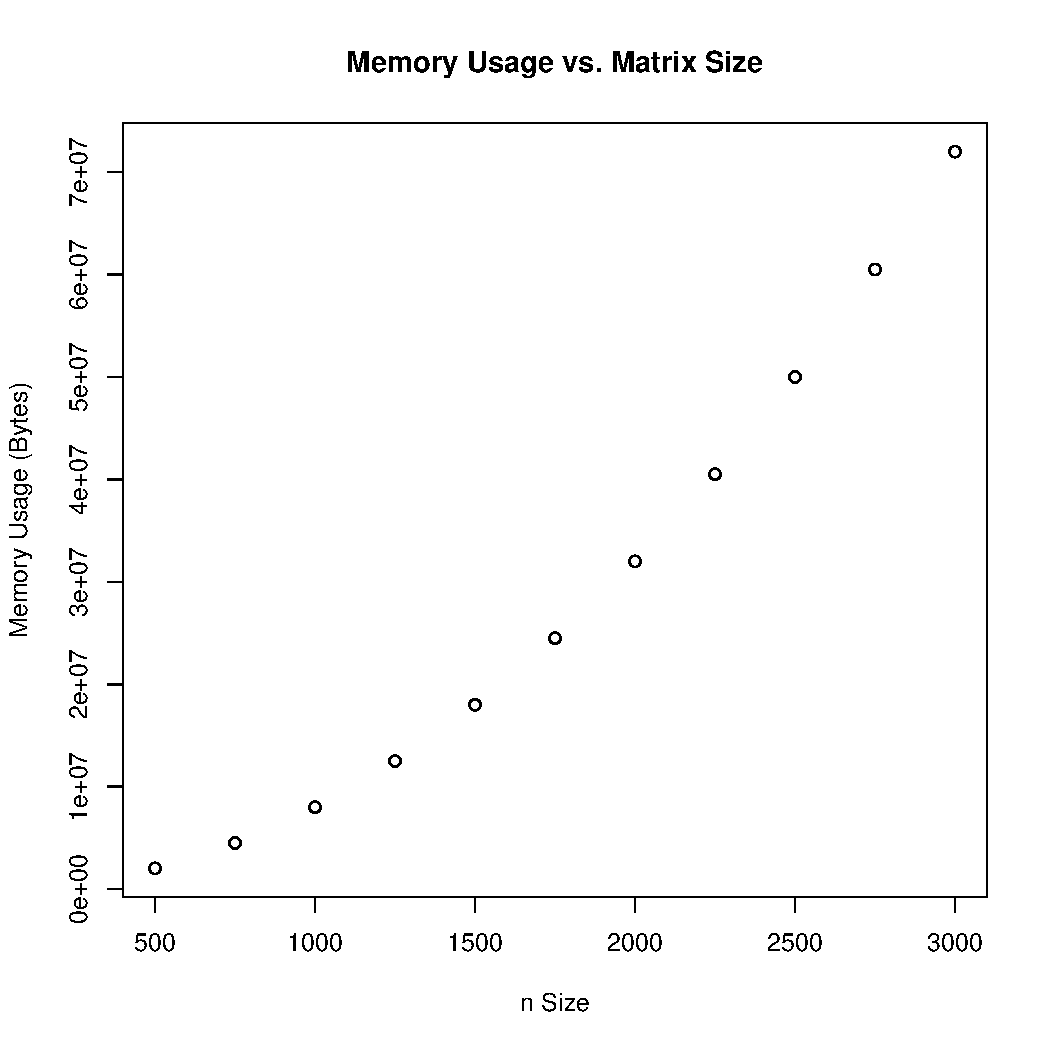
\includegraphics[width=\maxwidth]{figure/unnamed-chunk-1-1} 
\begin{kframe}\begin{alltt}
\hlkwd{plot}\hlstd{(}\hlkwc{x}\hlstd{=sizes,}\hlkwc{y}\hlstd{=times,}\hlkwc{xlab}\hlstd{=}\hlstr{"n Size"}\hlstd{,}\hlkwc{ylab}\hlstd{=}\hlstr{"Time (msec)"}\hlstd{,}\hlkwc{main}\hlstd{=}\hlstr{"Operation Time vs. Matrix Size"}\hlstd{)}
\end{alltt}
\end{kframe}
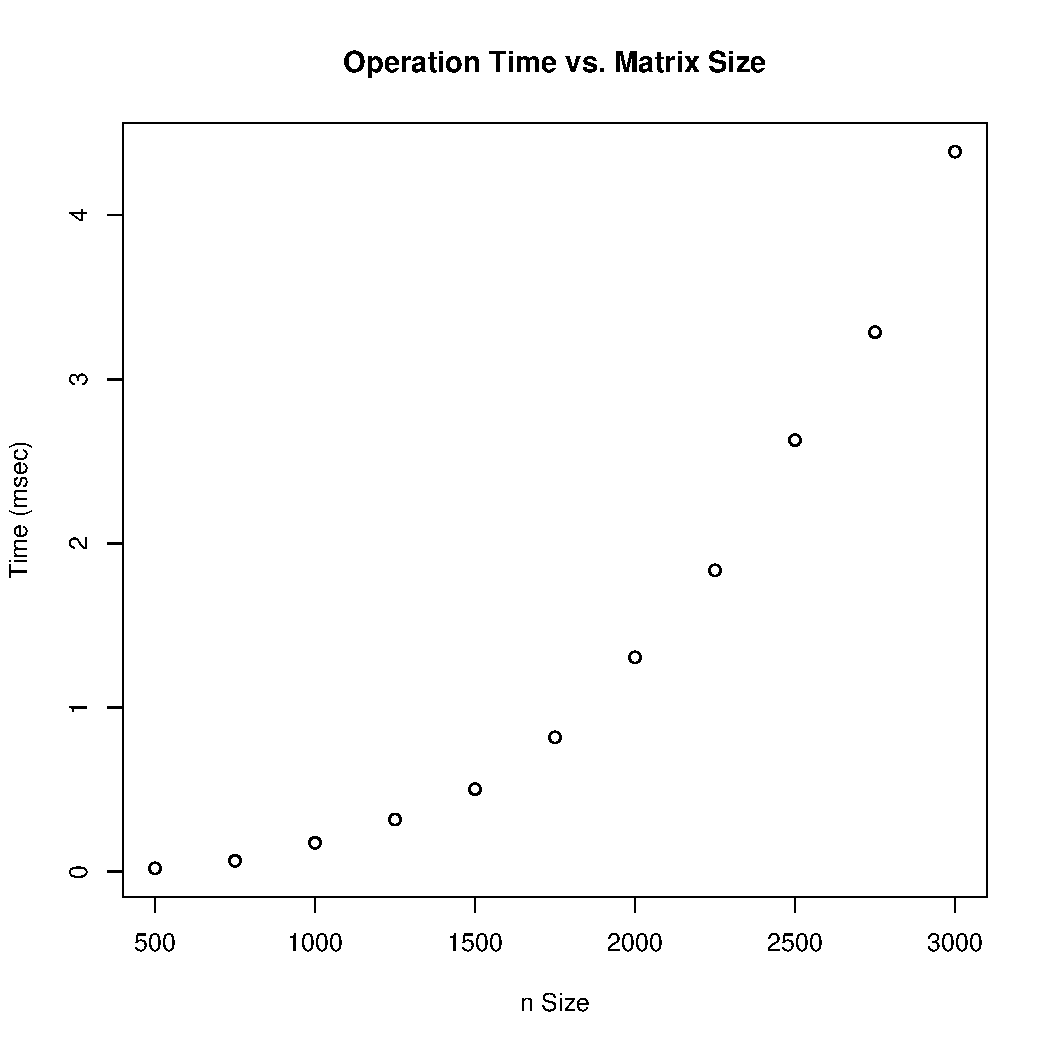
\includegraphics[width=\maxwidth]{figure/unnamed-chunk-1-2} 

\end{knitrout}

The values are scaling about \(O(n^3)\) which is roughly what we expect given the algorithm.

\section{}

\begin{knitrout}
\definecolor{shadecolor}{rgb}{0.969, 0.969, 0.969}\color{fgcolor}\begin{kframe}
\begin{alltt}
\hlkwd{set.seed}\hlstd{(}\hlnum{0}\hlstd{)}
\hlkwd{options}\hlstd{(}\hlkwc{digits}\hlstd{=}\hlnum{22}\hlstd{)}
\hlstd{N} \hlkwb{<-} \hlnum{5000}
\hlcom{# Initialize the pos-def matrix}
\hlstd{X} \hlkwb{<-} \hlkwd{crossprod}\hlstd{(}\hlkwd{matrix}\hlstd{(}\hlkwd{rnorm}\hlstd{(N}\hlopt{^}\hlnum{2}\hlstd{), N))}
\hlstd{y} \hlkwb{<-} \hlkwd{rnorm}\hlstd{(N)}

\hlkwd{print}\hlstd{(}\hlstr{"For the solve(X), then %*% method..."}\hlstd{)}
\end{alltt}
\begin{verbatim}
## [1] "For the solve(X), then %*% method..."
\end{verbatim}
\begin{alltt}
\hlkwd{system.time}\hlstd{(v1} \hlkwb{<-} \hlkwd{solve}\hlstd{(X)} \hlopt \hlstd{y)}
\end{alltt}
\begin{verbatim}
##                       user                     system 
## 250.4499999999999886313162   0.9560000000000001829648 
##                    elapsed 
## 252.2090000000000316049409
\end{verbatim}
\begin{alltt}
\hlkwd{print}\hlstd{(}\hlstr{"For the solve(X,y)..."}\hlstd{)}
\end{alltt}
\begin{verbatim}
## [1] "For the solve(X,y)..."
\end{verbatim}
\begin{alltt}
\hlkwd{system.time}\hlstd{(v2} \hlkwb{<-} \hlkwd{solve}\hlstd{(X,y))}
\end{alltt}
\begin{verbatim}
##                      user                    system 
## 28.1469999999999913598003  0.1129999999999999893419 
##                   elapsed 
## 28.3250000000000454747351
\end{verbatim}
\begin{alltt}
\hlkwd{print}\hlstd{(}\hlstr{"For the Cholesky decomposition..."}\hlstd{)}
\end{alltt}
\begin{verbatim}
## [1] "For the Cholesky decomposition..."
\end{verbatim}
\begin{alltt}
\hlkwd{system.time}\hlstd{(}
  \hlstd{\{}
    \hlcom{# Cholesky decompose, and then backsolve}
    \hlstd{U} \hlkwb{<-} \hlkwd{chol}\hlstd{(X);}
    \hlstd{v3} \hlkwb{<-} \hlkwd{backsolve}\hlstd{(U,} \hlkwd{backsolve}\hlstd{(U, y,} \hlkwc{transpose}\hlstd{=}\hlnum{TRUE}\hlstd{));}
  \hlstd{\}}
\hlstd{)}
\end{alltt}
\begin{verbatim}
##                      user                    system 
## 19.6909999999999740794010  0.1219999999999998863132 
##                   elapsed 
## 20.0880000000000222826202
\end{verbatim}
\begin{alltt}
\hlkwd{print}\hlstd{(}\hlstr{"Checking that our values are reasonable (i.e., the same)..."}\hlstd{)}
\end{alltt}
\begin{verbatim}
## [1] "Checking that our values are reasonable (i.e., the same)..."
\end{verbatim}
\begin{alltt}
\hlstd{v1[}\hlnum{1}\hlopt{:}\hlnum{10}\hlstd{]}
\end{alltt}
\begin{verbatim}
##  [1]  -4.803833033478003500250  17.758187412524087278598
##  [3] -19.910537805559485491358 -14.628034395977977055736
##  [5]  32.546734117480198733574  32.251918358480054394022
##  [7]  34.282461021149927660190 -73.309490570436381062791
##  [9] -20.014343424005812011046  -1.749447230489489468752
\end{verbatim}
\begin{alltt}
\hlstd{v2[}\hlnum{1}\hlopt{:}\hlnum{10}\hlstd{]}
\end{alltt}
\begin{verbatim}
##  [1]  -4.803833033477777902931  17.758187412523792403363
##  [3] -19.910537805559318513815 -14.628034395978076531719
##  [5]  32.546734117480127679300  32.251918358480033077740
##  [7]  34.282461021149750024506 -73.309490570436068423987
##  [9] -20.014343424005993199444  -1.749447230489707516554
\end{verbatim}
\begin{alltt}
\hlstd{v3[}\hlnum{1}\hlopt{:}\hlnum{10}\hlstd{]}
\end{alltt}
\begin{verbatim}
##  [1]  -4.803833043393967550116  17.758187421434300290457
##  [3] -19.910537817897626666763 -14.628034398574007113325
##  [5]  32.546734139602186530738  32.251918375158908247613
##  [7]  34.282461045482996553346 -73.309490601046292113097
##  [9] -20.014343430242931276553  -1.749447229275409743110
\end{verbatim}
\end{kframe}
\end{knitrout}

...Cholesky is defintely the fastest!  a) \(O(n^3)\) b) \( 1/3 n^3 + O(n^2) \) c) \(1/6 n^3 + O(n^2) \)  (source: the notes).  The timings generally agree.

\subsection{}

\begin{knitrout}
\definecolor{shadecolor}{rgb}{0.969, 0.969, 0.969}\color{fgcolor}\begin{kframe}
\begin{alltt}
\hlkwd{library}\hlstd{(MASS)}
\hlkwd{print}\hlstd{(}\hlstr{"Numerical differences between our answers"}\hlstd{)}
\end{alltt}
\begin{verbatim}
## [1] "Numerical differences between our answers"
\end{verbatim}
\begin{alltt}
\hlcom{# Max of differences between methods 1, 2 and 2, 3 and 3, 1 respectively}
\hlkwd{max}\hlstd{(}\hlkwd{abs}\hlstd{(v1}\hlopt{-}\hlstd{v2))}
\end{alltt}
\begin{verbatim}
## [1] 7.105427357601001858711e-13
\end{verbatim}
\begin{alltt}
\hlkwd{max}\hlstd{(}\hlkwd{abs}\hlstd{(v2}\hlopt{-}\hlstd{v3))}
\end{alltt}
\begin{verbatim}
## [1] 6.342163771932973759249e-08
\end{verbatim}
\begin{alltt}
\hlkwd{max}\hlstd{(}\hlkwd{abs}\hlstd{(v3}\hlopt{-}\hlstd{v1))}
\end{alltt}
\begin{verbatim}
## [1] 6.34216661410391679965e-08
\end{verbatim}
\begin{alltt}
\hlstd{a} \hlkwb{<-} \hlkwd{norm}\hlstd{(X,}\hlkwc{type}\hlstd{=}\hlstr{"2"}\hlstd{)} \hlopt{*} \hlkwd{norm}\hlstd{(}\hlkwd{ginv}\hlstd{(X),}\hlkwc{type}\hlstd{=}\hlstr{"2"}\hlstd{)}
\hlkwd{print}\hlstd{(}\hlstr{"The Condition Number"}\hlstd{)}
\end{alltt}
\begin{verbatim}
## [1] "The Condition Number"
\end{verbatim}
\begin{alltt}
\hlkwd{print}\hlstd{(a} \hlopt{*} \hlnum{1e-16}\hlstd{)}
\end{alltt}
\begin{verbatim}
## [1] 4.029048851270799130557e-09
\end{verbatim}
\end{kframe}
\end{knitrout}

The differences are really not that pronounced.  This agrees with the relative numerical stability assured by the condition number.

\section{}

The general scheme and pseudocode for the matrix manipulations used was as follows:\\

Given:

\[ \hat{\beta} = \left( X^T \Sigma^{-1} X \right)^{-1} X^T \Sigma^{-1} Y \]

We use eigenvectors and eigenvalues to rewrite sigma inverse as:

\[ \Sigma^{-1} = C \Lambda C^{-1} \]

Which we can further simply to:

\[ \Sigma^{-1} = P P^T \]

Where:

\[ P = C \Lambda^{1/2} \]

This allows us to transform X and Y, so the QR decomposition can be performed, so that our calculation is of an acceptable speed:

\[X_* = P^T X\]

and

\[Y_* = P^T Y \]

Now we follow a QR decomposition, much like in the notes with OLE:

\[X_*^T X_* \hat \beta = X_*^T Y \]

\[R^T Q^T Q R \hat \beta = R^T Q^T Y_*\]

And we can use back solving to find:

\[ R \hat \beta = Q^T Y_* \]

\begin{knitrout}
\definecolor{shadecolor}{rgb}{0.969, 0.969, 0.969}\color{fgcolor}\begin{kframe}
\begin{alltt}
\hlkwd{library}\hlstd{(MASS)}
\hlstd{n} \hlkwb{<-} \hlnum{50}
\hlstd{p} \hlkwb{<-} \hlnum{10}

\hlstd{X} \hlkwb{<-} \hlkwd{matrix}\hlstd{(}\hlkwd{runif}\hlstd{(n}\hlopt{*}\hlstd{p),} \hlkwc{ncol}\hlstd{=p)}
\hlstd{Sigma} \hlkwb{<-} \hlkwd{crossprod}\hlstd{(}\hlkwd{matrix}\hlstd{(}\hlkwd{rnorm}\hlstd{(n}\hlopt{^}\hlnum{2}\hlstd{), n))}
\hlstd{Y} \hlkwb{<-} \hlkwd{matrix}\hlstd{(}\hlkwd{runif}\hlstd{(n),} \hlkwc{ncol}\hlstd{=}\hlnum{1}\hlstd{)}

\hlstd{my_gls} \hlkwb{<-} \hlkwa{function}\hlstd{(}\hlkwc{X}\hlstd{,} \hlkwc{Sigma}\hlstd{,} \hlkwc{Y}\hlstd{,} \hlkwc{n}\hlstd{,} \hlkwc{p}\hlstd{) \{}
    \hlcom{# Generate sigma inverse}
    \hlstd{Sigma_inv} \hlkwb{<-} \hlkwd{ginv}\hlstd{(Sigma)}
    \hlcom{# Eigendecompose sigma inverse}
    \hlstd{Sigma_inv_eigen_object} \hlkwb{<-} \hlkwd{eigen}\hlstd{(Sigma_inv)}
    \hlstd{P} \hlkwb{<-} \hlstd{Sigma_inv_eigen_object}\hlopt{$}\hlstd{vectors} \hlopt
      \hlkwd{diag}\hlstd{(}\hlkwd{sqrt}\hlstd{(Sigma_inv_eigen_object}\hlopt{$}\hlstd{values))}
    \hlstd{Pt} \hlkwb{<-} \hlkwd{t}\hlstd{(P)}
    \hlcom{# Generate our Y/X "stars" form the pseudocode}
    \hlstd{Y_mod} \hlkwb{<-} \hlstd{Pt} \hlopt \hlstd{Y}
    \hlstd{X_mod} \hlkwb{<-} \hlstd{Pt} \hlopt \hlstd{X}
    \hlcom{# Perform a QR decomposition}
    \hlstd{X_mod.qr} \hlkwb{<-} \hlkwd{qr}\hlstd{(X_mod)}
    \hlstd{Q} \hlkwb{<-} \hlkwd{qr.Q}\hlstd{(X_mod.qr)}
    \hlstd{R} \hlkwb{<-} \hlkwd{qr.R}\hlstd{(X_mod.qr)}
    \hlcom{# Backsolve, and return the values}
    \hlkwd{return}\hlstd{(}\hlkwd{backsolve}\hlstd{(R,} \hlkwd{t}\hlstd{(Q)} \hlopt \hlstd{Y_mod))}
\hlstd{\}}

\hlkwd{print}\hlstd{(}\hlkwd{my_gls}\hlstd{(X, Sigma, Y, n, p))}
\end{alltt}
\begin{verbatim}
##                             [,1]
##  [1,] -0.38178770437887171729230
##  [2,]  0.43199236710490312995958
##  [3,] -0.06137662709808201083606
##  [4,]  0.60279399525459143038830
##  [5,] -0.47983751521344436552496
##  [6,] -0.01672323669622955907843
##  [7,] -0.14536684054820322997692
##  [8,] -0.03198516007207349159946
##  [9,]  0.03981707405928997661748
## [10,]  1.07242103894418416842882
\end{verbatim}
\begin{alltt}
\hlcom{# Checking our answer against the "long" way...}
\hlcom{# This was the problem statement (but too slow for our solution)}

\hlstd{Sigma_inv} \hlkwb{<-} \hlkwd{ginv}\hlstd{(Sigma)}
\hlkwd{ginv}\hlstd{(}\hlkwd{t}\hlstd{(X)} \hlopt \hlstd{Sigma_inv} \hlopt \hlstd{X)} \hlopt \hlkwd{t}\hlstd{(X)} \hlopt \hlstd{Sigma_inv} \hlopt \hlstd{Y}
\end{alltt}
\begin{verbatim}
##                             [,1]
##  [1,] -0.38178770437844999907639
##  [2,]  0.43199236710481431211761
##  [3,] -0.06137662709890697593229
##  [4,]  0.60279399525442456386770
##  [5,] -0.47983751521576090137700
##  [6,] -0.01672323669648601018878
##  [7,] -0.14536684054862153425702
##  [8,] -0.03198516006718693516220
##  [9,]  0.03981707406077009125944
## [10,]  1.07242103894115814455290
\end{verbatim}
\end{kframe}
\end{knitrout}

\section{}

\subsection{}

Suppose we write X as:

\[ X = U_{n x n} S_{n x p} V^T_{p x p} \]

Manipulate further:

\begin{align*}
X^T &= (USV^T)^T\\
    &= VS^TU^T\\
X^TX &= VS^TU^TUSV^T\\
     &= VS^TISV^T
\end{align*}

S is diagonalizable, so \(S^T = S\):

\[ X^TX = VS^2V^T \]

So our eigenvectors are \(V\) and \(V^T\) -- the right singular vecotrs of X.  We can also see that \(S^2\) are the eigenvalues -- the square of the singular values of X.\\\\

We now show that \(XX^T\) is positive semidefinite.  Take v s.t. \(v_i \neq 0 \forall i\):

\begin{align*}
v^t X^T X v &= (vX)^T X v\\
            &= s^T s\\
            &= \sum s_i^2 \ge 0
\end{align*}

Sources: Dug through some econometrics notes as well as a linear algebra textbook my roommate had lying around.

\begin{knitrout}
\definecolor{shadecolor}{rgb}{0.969, 0.969, 0.969}\color{fgcolor}\begin{kframe}
\begin{alltt}
\hlstd{n} \hlkwb{<-} \hlnum{1000}
\hlstd{p} \hlkwb{<-} \hlnum{500}

\hlstd{X} \hlkwb{<-} \hlkwd{matrix}\hlstd{(}\hlkwd{runif}\hlstd{(n}\hlopt{*}\hlstd{p),} \hlkwc{ncol}\hlstd{=p)}
\hlstd{eigen_object} \hlkwb{<-} \hlkwd{eigen}\hlstd{(}\hlkwd{t}\hlstd{(X)} \hlopt \hlstd{X)}
\hlstd{X_svd} \hlkwb{<-} \hlkwd{svd}\hlstd{(X)}

\hlcom{# Are the right singular vectors of X equal to}
\hlcom{# the eigenvectors of X^t * X?}

\hlkwd{print}\hlstd{(}\hlstr{"Right Singular Vectors of X..."}\hlstd{)}
\end{alltt}
\begin{verbatim}
## [1] "Right Singular Vectors of X..."
\end{verbatim}
\begin{alltt}
\hlkwd{head}\hlstd{(X_svd}\hlopt{$}\hlstd{v[,}\hlnum{1}\hlopt{:}\hlnum{10}\hlstd{])}
\end{alltt}
\begin{verbatim}
##             [,1]          [,2]         [,3]        [,4]         [,5]
## [1,] -0.04431472 -0.0713039531  0.015694327 -0.09116894  0.039093598
## [2,] -0.04550727  0.0987448093 -0.049431463  0.06035542 -0.013809752
## [3,] -0.04475009  0.0550687752 -0.006895094 -0.04915989  0.019327870
## [4,] -0.04464549  0.0653306270  0.025773791  0.02762509 -0.029110710
## [5,] -0.04390919 -0.0084620402  0.092150351 -0.07410252 -0.052462206
## [6,] -0.04438632  0.0009634196 -0.098575350  0.04329162 -0.008783357
##              [,6]         [,7]        [,8]          [,9]        [,10]
## [1,] -0.008111073  0.023962732 -0.10558649  2.613512e-02 -0.033087289
## [2,]  0.025553020  0.001906576  0.02446195 -4.220050e-03 -0.053928820
## [3,]  0.048226365 -0.094035323 -0.02009505  7.209434e-06  0.032340415
## [4,]  0.020982967 -0.035142588  0.02920922 -6.258991e-02 -0.009316251
## [5,]  0.040685745 -0.034828816  0.04830455 -5.505051e-02 -0.027224582
## [6,]  0.051545496 -0.024424176  0.02181362  8.102247e-02 -0.025520552
\end{verbatim}
\begin{alltt}
\hlkwd{print}\hlstd{(}\hlstr{"Eigenvectors of X^t * X"}\hlstd{)}
\end{alltt}
\begin{verbatim}
## [1] "Eigenvectors of X^t * X"
\end{verbatim}
\begin{alltt}
\hlkwd{head}\hlstd{(eigen_object}\hlopt{$}\hlstd{vectors[,}\hlnum{1}\hlopt{:}\hlnum{10}\hlstd{])}
\end{alltt}
\begin{verbatim}
##             [,1]          [,2]         [,3]        [,4]         [,5]
## [1,] -0.04431472  0.0713039531  0.015694327 -0.09116894 -0.039093598
## [2,] -0.04550727 -0.0987448093 -0.049431463  0.06035542  0.013809752
## [3,] -0.04475009 -0.0550687752 -0.006895094 -0.04915989 -0.019327870
## [4,] -0.04464549 -0.0653306270  0.025773791  0.02762509  0.029110710
## [5,] -0.04390919  0.0084620402  0.092150351 -0.07410252  0.052462206
## [6,] -0.04438632 -0.0009634196 -0.098575350  0.04329162  0.008783357
##              [,6]         [,7]        [,8]          [,9]        [,10]
## [1,] -0.008111073  0.023962732  0.10558649 -2.613512e-02 -0.033087289
## [2,]  0.025553020  0.001906576 -0.02446195  4.220050e-03 -0.053928820
## [3,]  0.048226365 -0.094035323  0.02009505 -7.209434e-06  0.032340415
## [4,]  0.020982967 -0.035142588 -0.02920922  6.258991e-02 -0.009316251
## [5,]  0.040685745 -0.034828816 -0.04830455  5.505051e-02 -0.027224582
## [6,]  0.051545496 -0.024424176 -0.02181362 -8.102247e-02 -0.025520552
\end{verbatim}
\begin{alltt}
\hlcom{# Are the eigenvalues of X^t * X equal to the }
\hlcom{# squares of the singular values of X?}

\hlkwd{print}\hlstd{(}\hlstr{"Eigenvalues of X^t * X"}\hlstd{)}
\end{alltt}
\begin{verbatim}
## [1] "Eigenvalues of X^t * X"
\end{verbatim}
\begin{alltt}
\hlkwd{head}\hlstd{(eigen_object}\hlopt{$}\hlstd{values)}
\end{alltt}
\begin{verbatim}
## [1] 125215.5298    239.2660    237.1677    235.4653    231.5683    228.7211
\end{verbatim}
\begin{alltt}
\hlkwd{print}\hlstd{(}\hlstr{"Squared singular values of X"}\hlstd{)}
\end{alltt}
\begin{verbatim}
## [1] "Squared singular values of X"
\end{verbatim}
\begin{alltt}
\hlkwd{head}\hlstd{(X_svd}\hlopt{$}\hlstd{d}\hlopt{**}\hlnum{2}\hlstd{)}
\end{alltt}
\begin{verbatim}
## [1] 125215.5298    239.2660    237.1677    235.4653    231.5683    228.7211
\end{verbatim}
\begin{alltt}
\hlcom{# Is X' * X a positive semidefinite matrix?}

\hlkwd{library}\hlstd{(}\hlstr{"matrixcalc"}\hlstd{)}
\hlkwd{print}\hlstd{(}\hlstr{"Is X' * X a positive semidefinite matrix?"}\hlstd{)}
\end{alltt}
\begin{verbatim}
## [1] "Is X' * X a positive semidefinite matrix?"
\end{verbatim}
\begin{alltt}
\hlkwd{is.positive.semi.definite}\hlstd{(}\hlkwd{t}\hlstd{(X)} \hlopt \hlstd{X)}
\end{alltt}
\begin{verbatim}
## [1] TRUE
\end{verbatim}
\end{kframe}
\end{knitrout}

\subsection{}

Now we consider an n x n positive semi-definite matrix X and assume we have already computed the eigendecomposition.
\begin{align*}
XDX^T + Ic &= XDX^T + XcX^T\\
           &= X(D + cI)X^T
\end{align*}

Some code illustrating our proof(s):

\begin{knitrout}
\definecolor{shadecolor}{rgb}{0.969, 0.969, 0.969}\color{fgcolor}\begin{kframe}
\begin{alltt}
\hlstd{N} \hlkwb{<-} \hlnum{10}
\hlstd{X} \hlkwb{<-} \hlkwd{crossprod}\hlstd{(}\hlkwd{matrix}\hlstd{(}\hlkwd{rnorm}\hlstd{(N}\hlopt{^}\hlnum{2}\hlstd{), N))}
\hlcom{# Store our eigenvalues for later}
\hlstd{eigen_objects} \hlkwb{<-} \hlkwd{eigen}\hlstd{(X)}

\hlcom{# Create Z from X and cI}
\hlstd{Z} \hlkwb{<-} \hlstd{X} \hlopt{+} \hlkwd{diag}\hlstd{(N)} \hlopt{*} \hlkwd{rep}\hlstd{(}\hlnum{2}\hlstd{,}\hlnum{10}\hlstd{)}
\hlstd{Z_eigen_objects} \hlkwb{<-} \hlkwd{eigen}\hlstd{(Z)}

\hlcom{# So slow!  Our "truth" to compare against}
\hlstd{Z_eigen_objects}\hlopt{$}\hlstd{values}
\end{alltt}
\begin{verbatim}
##  [1] 25.575519 23.419765 17.188487 12.155543 10.797895  9.377336  4.723900
##  [8]  3.225932  2.450137  2.038489
\end{verbatim}
\begin{alltt}
\hlcom{# Order O(n)... much faster!}
\hlstd{eigen_objects}\hlopt{$}\hlstd{values} \hlopt{+} \hlkwd{rep}\hlstd{(}\hlnum{2}\hlstd{,}\hlnum{10}\hlstd{)}
\end{alltt}
\begin{verbatim}
##  [1] 25.575519 23.419765 17.188487 12.155543 10.797895  9.377336  4.723900
##  [8]  3.225932  2.450137  2.038489
\end{verbatim}
\end{kframe}
\end{knitrout}

\end{document}
